\def\year{2022}\relax
%File: formatting-instructions-latex-2022.tex
%release 2022.1
\documentclass[letterpaper]{article} % DO NOT CHANGE THIS
\usepackage{aaai22}  % DO NOT CHANGE THIS
\usepackage{times}  % DO NOT CHANGE THIS
\usepackage{helvet}  % DO NOT CHANGE THIS
\usepackage{courier}  % DO NOT CHANGE THIS
\usepackage[hyphens]{url}  % DO NOT CHANGE THIS
\usepackage{graphicx} % DO NOT CHANGE THIS
\urlstyle{rm} % DO NOT CHANGE THIS
\def\UrlFont{\rm}  % DO NOT CHANGE THIS
\usepackage{natbib}  % DO NOT CHANGE THIS AND DO NOT ADD ANY OPTIONS TO IT
\usepackage{caption} % DO NOT CHANGE THIS AND DO NOT ADD ANY OPTIONS TO IT
\DeclareCaptionStyle{ruled}{labelfont=normalfont,labelsep=colon,strut=off} % DO NOT CHANGE THIS
\frenchspacing  % DO NOT CHANGE THIS
\setlength{\pdfpagewidth}{8.5in}  % DO NOT CHANGE THIS
\setlength{\pdfpageheight}{11in}  % DO NOT CHANGE THIS
%
% These are recommended to typeset algorithms but not required. See the subsubsection on algorithms. Remove them if you don't have algorithms in your paper.
\usepackage{algorithm}
\usepackage{algpseudocode}

%
% These are are recommended to typeset listings but not required. See the subsubsection on listing. Remove this block if you don't have listings in your paper.
\usepackage{newfloat}
\usepackage{listings}
\lstset{%
	basicstyle={\footnotesize\ttfamily},% footnotesize acceptable for monospace
	numbers=left,numberstyle=\footnotesize,xleftmargin=2em,% show line numbers, remove this entire line if you don't want the numbers.
	aboveskip=0pt,belowskip=0pt,%
	showstringspaces=false,tabsize=2,breaklines=true}
\floatstyle{ruled}
\newfloat{listing}{tb}{lst}{}
\floatname{listing}{Listing}

\usepackage{amsfonts}
\usepackage{amsmath}
\DeclareMathOperator*{\argmin}{arg\,min}
\DeclareMathOperator*{\argmax}{arg\,max}
\renewcommand{\Return}[1]{\State \textbf{return} #1}

\usepackage{hyperref}

\graphicspath{{./img/}}

%
%\nocopyright
%
% PDF Info Is REQUIRED.
% For /Title, write your title in Mixed Case.
% Don't use accents or commands. Retain the parentheses.
% For /Author, add all authors within the parentheses,
% separated by commas. No accents, special characters
% or commands are allowed.
% Keep the /TemplateVersion tag as is
\pdfinfo{
/Title (Playing Tetris With Monte Carlo Tree Search)
/Author (Mike Delmonaco)
/TemplateVersion (2022.1)
}

% DISALLOWED PACKAGES
% \usepackage{authblk} -- This package is specifically forbidden
% \usepackage{balance} -- This package is specifically forbidden
% \usepackage{color (if used in text)
% \usepackage{CJK} -- This package is specifically forbidden
% \usepackage{float} -- This package is specifically forbidden
% \usepackage{flushend} -- This package is specifically forbidden
% \usepackage{fontenc} -- This package is specifically forbidden
% \usepackage{fullpage} -- This package is specifically forbidden
% \usepackage{geometry} -- This package is specifically forbidden
% \usepackage{grffile} -- This package is specifically forbidden
% \usepackage{hyperref} -- This package is specifically forbidden
% \usepackage{navigator} -- This package is specifically forbidden
% (or any other package that embeds links such as navigator or hyperref)
% \indentfirst} -- This package is specifically forbidden
% \layout} -- This package is specifically forbidden
% \multicol} -- This package is specifically forbidden
% \nameref} -- This package is specifically forbidden
% \usepackage{savetrees} -- This package is specifically forbidden
% \usepackage{setspace} -- This package is specifically forbidden
% \usepackage{stfloats} -- This package is specifically forbidden
% \usepackage{tabu} -- This package is specifically forbidden
% \usepackage{titlesec} -- This package is specifically forbidden
% \usepackage{tocbibind} -- This package is specifically forbidden
% \usepackage{ulem} -- This package is specifically forbidden
% \usepackage{wrapfig} -- This package is specifically forbidden
% DISALLOWED COMMANDS
% \nocopyright -- Your paper will not be published if you use this command
% \addtolength -- This command may not be used
% \balance -- This command may not be used
% \baselinestretch -- Your paper will not be published if you use this command
% \clearpage -- No page breaks of any kind may be used for the final version of your paper
% \columnsep -- This command may not be used
% \newpage -- No page breaks of any kind may be used for the final version of your paper
% \pagebreak -- No page breaks of any kind may be used for the final version of your paperr
% \pagestyle -- This command may not be used
% \tiny -- This is not an acceptable font size.
% \vspace{- -- No negative value may be used in proximity of a caption, figure, table, section, subsection, subsubsection, or reference
% \vskip{- -- No negative value may be used to alter spacing above or below a caption, figure, table, section, subsection, subsubsection, or reference

\setcounter{secnumdepth}{0} %May be changed to 1 or 2 if section numbers are desired.

% The file aaai22.sty is the style file for AAAI Press
% proceedings, working notes, and technical reports.
%

% Title

% Your title must be in mixed case, not sentence case.
% That means all verbs (including short verbs like be, is, using,and go),
% nouns, adverbs, adjectives should be capitalized, including both words in hyphenated terms, while
% articles, conjunctions, and prepositions are lower case unless they
% directly follow a colon or long dash
\title{Playing Tetris With Monte Carlo Tree Search}
\author{
    %Authors
    % All authors must be in the same font size and format.
    Mike Delmonaco
}
\affiliations{
    %Afiliations
  Northeastern University\\
  delmonaco.m@northeastern.edu
% See more examples next
}

%Example, Single Author, ->> remove \iffalse,\fi and place them surrounding AAAI title to use it
\iffalse
\title{My Publication Title --- Single Author}
\author {
    Author Name
}
\affiliations{
    Affiliation\\
    Affiliation Line 2\\
    name@example.com
}
\fi

\iffalse
%Example, Multiple Authors, ->> remove \iffalse,\fi and place them surrounding AAAI title to use it
\title{My Publication Title --- Multiple Authors}
\author {
    % Authors
    First Author Name,\textsuperscript{\rm 1}
    Second Author Name, \textsuperscript{\rm 2}
    Third Author Name \textsuperscript{\rm 1}
}
\affiliations {
    % Affiliations
    \textsuperscript{\rm 1} Affiliation 1\\
    \textsuperscript{\rm 2} Affiliation 2\\
    firstAuthor@affiliation1.com, secondAuthor@affilation2.com, thirdAuthor@affiliation1.com
}
\fi

\begin{document}

\newcommand{\tetris}{\emph{Tetris}}

\maketitle

\begin{abstract}
  \tetris{} is a puzzle video game that involves moving differently shaped pieces as they fall in a grid.
  \tetris{} is a difficult problem for AI, mainly because of its large state space and the long term planning required to survive and play well.
  Monte Carlo tree search is well-suited for both of these issues. In this paper, I apply Monte Carlo tree search to \tetris. Several configurations and variants are explored and compared to simple baselines.
  I found that the highest-performing Monte Carlo tree search agent performs slightly worse than the heuristic minimax baseline agents.

  The source code for the environment, agents, and experiments are available on GitHub \footnote{https://github.com/quasarbright/TetrisAI}.
\end{abstract}

\section{Introduction}
The game \tetris{} involves moving differently shaped pieces as they fall in a grid.
The objective of \tetris{} is to arrange pieces such that they form a complete row of squares. This removes the row and grants score. The game ends when the pieces get stacked so high that a new piece doesn't have room to spawn at the top of the grid.
As the player earns more score, the player's level increases. As the level increases, the rate at which pieces fall after spawning increases, giving the player less time to think and maneuver the piece.
The fastest way to earn score is to clear 4 lines at ones with a vertical line piece. This is called a tetris.

\tetris{} is a difficult problem to solve with AI for a few reasons:

\begin{itemize}
  \item{
        Careful, long-term planning is required to perform a tetris. The player must arrange the pieces in such a way that 4 rows are
        filled, except for one vertical well that must not be covered from above to prevent a line piece from falling into the well. Since the play field's grid is 10 squares wide and each piece occupies 4 squares, creating this well requires at least
        nine pieces, and an additional line piece to perform the tetris. This means any tree-search-like agent must plan at least ten pieces ahead in order to see the possibility of a tetris. Additionally, even to simply survive, long-term planning is
        necessary. It can take a long time to recover from a misplaced piece that prevents the player from clearing a line. If lines aren't cleared, the grid fills up an the player loses.
        }
  \item{
        \tetris{} is played in a grid that is 10 squares wide and at least 20 squares tall (height varies between versions of the game) and each cell may or may not be occupied by a square from one of the falling pieces. This means there are at least \(2^{200}\)
        possible states. Thus, dynamic programming and tabular methods would be very inefficient.
        }
  \item{
        Due to ``gravity'' increasing as the level number increases, the environment is non-stationary. However, it is possible to formulate the problem as a stationary MDP if the level is considered part of the state.
        }
  \item{
        The environment is stochastic since the sequence of pieces is generated randomly.
        }
\end{itemize}

Monte Carlo tree search is method that is suitable for all of these challenging aspects of the problem. It is capable of efficient long-term planning, can handle large state spaces, non-stationary environments, and stochastic environments.

\section{Background}

\subsection{Tree Search Methods}
Tree search methods are useful for MDPs with large state spaces. These methods require a simulator of the environment that is capable of playing out multiple possible actions from a state. In general, tree search methods start at the current state,
try some actions which yield next states, and recur on those next states. They try many different possible sequences of actions and, after a certain number of iterations, choose the ``best'' action in some sense. A simple example
is minimax, which tries every possible sequence of actions from the current state. Each sequence of actions has some value. For a MDP, this could be the return along the sequence. The next action taken is the first action of the maximum-valued sequence.

Minimax is a very simple and straightforward algorithm, but it is inefficient for high search depths. The asymptotic time complexity of minimax is \(O(b^{d})\), where \(b\) is the number of possible actions at each timestep and \(d\) is the depth
of the search. Often times, rather than searching to the end of an episode, the search is limited to a certain number of timesteps. This means the optimal action may not be chosen, but computation time is significantly reduced.

Another common augmentation is using a heuristic to evaluate the final state of a search branch, rather than using the return. The goal is still to optimize the return, but a shallow search optimizing a heuristic designed by domain experts can perform
very well.

\subsection{Upper Confidence Bounds}

In many RL methods, there is a tradeoff between exploration and exploitation while learning and/or planning. Should the agent explore unseen states and see if there is anything better than what it has experienced? Or should the agent exploit what it has
learned and follow the path which seems best with its current knowledge? One method to find a balance between these two options is the upper confidence bound (UCB) algorithm. This method is applicable to multi-armed bandit problems and uses the following
equation to select actions:

\[A_{t} = \argmax_{a}\left[Q_{t}(a) + c \sqrt{\frac{\log t}{N_{t}(a)}}\right]\]

\noindent{}
where \(c\) is is a hyperparameter that controls the strength of the exploration bonus, \(t\) is the current timestep, and \(N_{t}(a)\) is the number of times the action has been performed.

This equation encourages exploration initially, but the exploration bonus diminishes over time since the numerator of the exploration bonus term grows logarithmically with respect to time and the denominator grows linearly. There will always be some exploration, but it will
decrease over time. This is exactly what we want for an agent ``learning as it goes''. Initially, it should favor exploration to experience the possibilities, but later, it should become more confident in its knowledge and exploit it.

\section{Related Work}

Tabular planning methods like DynaQ can be useful for a problem that requires planning. However, tabular methods rely on learning a value associated with each state
or state-action pair. Since the state space is so large, it is impractical to try to store information about every state in memory. Furthermore, since states are unlikely to ever repeat within or across episodes, tabular methods would require many episodes to learn anything applicable to future episodes. Even if the method has planning steps like DynaQ which replay episodes, since states are unlikely to repeat in the future, most of the time, the agent will always be experiencing a state for the first time and never
use anything it has learned. There are just too many different states and the agent has no way of using what it learned in one state and applying it to another state. This could be accomplished with feature engineering, but that would require great effort from domain experts. Far more than what is required for a state evaluation heuristic. Monte Carlo tree search is also a planning method, but it is more well-suited for problems with large, non-repeating state spaces.

One alternative method that could be applied to this problem is minimax. Minimax, the tree search algorithm described in the previous section, is well-suited for problems with large state spaces. However, its runtime is exponential in the search depth, making it impractical for problems which require long-term planning. One popular augmentation to reduce the search space is alpha-beta pruning, but unfortunately, it is not applicable to single player games. Monte Carlo tree search is also a tree search method, but it prunes most of the search space by focusing on promising nodes.

\section{Project Description}

\subsection{Markov Decision Process Formulation}
\tetris{} can be formulated as an MDP, represented by the tuple \((\mathcal{S}, \mathcal{A}, \mathcal{T}, \mathcal{R})\) representing the set of states, set of actions, transition function, and reward function.
Each state is described by the following pieces of data:

\begin{itemize}
  \item{
        For each grid cell, a bit, where zero represents an unoccupied cell and one represents an occupied cell.
        }
  \item{
        The shape, position, and rotation of the current piece
        }
  \item{
        The sequence of three previewed piece shapes
        }
  \item{
        The current level number
        }
  \item{
        A bit representing whether the game has ended, where zero represents an unfinished game and 1 represents a game that has ended from the player losing.
        }
\end{itemize}

The grid has 10 columns and 20 rows. There are seven piece shapes: I, O, T, S, Z, J, and L. The level number is an integer greater than or equal to six. There is no upper bound. This means, theoretically, the state space is infinite. In practice,
levels after a certain point (level 29) behave identically. The only thing that changes between levels is the speed at which pieces fall. After level 29, they fall at an entire screen per frame. Levels after this techincally have a higher falling speed,
but they behave identically. The formulation used in this paper is chosen to mimic what a human would be able to know by looking at a single frame of the screen without having deep knowledge of the game's rules.

There are two formulations of actions that are used in this paper: A low-level raw input formulation that mimics a human's available actions, and a high-level formulation engineered to aid tree searches.

A low-level action is one of ``move left'', ``move right'', ``rotate counter clockwise'', ``rotate clockwise'', ``soft drop'', ``hard drop'', or ``do nothing''.

A high-level action consists of a horizontal shift and a rotation, which are integers in the ranges \([-5,5]\) and \([0,3]\) respectively, representing the position and orientation at which a piece is placed.

The transition function is very complicated, with many edge cases. The \tetris{} guideline\footnote{\url{https://tetris.wiki/Tetris_Guideline}} specifies the rules for how pieces move and rotate, scoring, etc. To summarize the relevant rules:

\begin{itemize}
  \item{
        Pressing the ``move left'' or ``move right'' inputs move the current piece horizontally one square.
        }
  \item{
        Pressing the ``rotate clockwise'' or ``rotate counter-clockwise'' inputs rotate the current piece.
        }
  \item{
        Pressing and holding the ``soft drop'' input causes the current piece to fall more quickly.
        }
  \item{
        Pressing the ``hard drop'' input causes the current piece to instantly fall and lock into the grid.
        }
  \item{
        When a piece falls to the grid and is on top of an occupied cell, after 30 frames of not moving, it locks into the grid and the next piece begins to fall.
        }
  \item{
        When a piece locking into the grid causes a row or rows to be completely occupied, it is removed and the grid above it shifts down to replace it.
        }
  \item{
        After a certain number of line clears, the level number increments.
        }
  \item{
        The sequence of next piece shapes is generated randomly.
        }
  \item{
        If a piece spawns and any of its squares are in a position that corresponds to an occupied grid cell, the game ends.
        }
\end{itemize}

The reward is zero for all state-action pairs, except for entering a terminal state (one where the bit representing a game's end is one), where it is the in-game score. The in-game score is also quite complicated, and is summarized by the following relevant details:

\begin{itemize}
  \item{
        Score is rewarded while the current piece falls.
        }
  \item{
        More score is rewarded for falling while soft dropping.
        }
  \item{
        For hard dropping, the score increases more than if the player soft dropped or let the piece fall naturally.
        }
  \item{
        Score is rewarded for clearing lines. More score is rewarded for clearing multiple lines with a single piece.
        }
\end{itemize}

There is no discounting.

\subsection{Monte Carlo Tree Search}

\begin{algorithm}
\caption{Monte Carlo tree search}
\label{alg:mcts}
\textbf{Input}: $S_{0} \in \mathcal{S}$\\
\textbf{Parameter}: $n \in \mathbb{N}$ number of iterations to perform\\
\textbf{Output}: The next action to take
\begin{algorithmic}[1] %[1] enables line numbers
\State $N(s,a) \gets 0\ \forall s \in \mathcal{S}, a \in \mathcal{A}$\Comment{Number of visits}
\State $N(s) \gets 0\ \forall s \in \mathcal{S}$
\State $T(s,a) \gets 0\ \forall s \in \mathcal{S}, a \in \mathcal{A}$\Comment{Total return}
\For{$n$ iterations}
  \State $\mathrm{pairs},S_{\mathrm{rollout}} \gets \Call{SelectExpand}{S_{0}}$
  \State $G \gets \Call{Rollout}{S_{\mathrm{rollout}}}$
  \State $\Call{Backup}{\mathrm{pairs}, G}$
\EndFor
\Return{$\argmax_{a}\frac{T(s,a)}{N(s,a)}$}

\Procedure{SelectExpand}{$s$}
  \State $\mathrm{pairs} \gets []$
  \Repeat
    \State $a \gets$ choose action using selection policy
    \State $\mathrm{pairs} \gets \mathrm{pairs}, (s,a)$
    \State $s,r \gets \Call{Step}{s,a}$
  \Until{$N(s) = 0$ or $s$ is terminal}
  \Return{$\mathrm{pairs}, s$}
\EndProcedure

\Procedure{Rollout}{$s$}
  \Repeat
    \State $a \gets$ choose action using rollout policy
    \State $s,r \gets \Call{Step}{s,a}$
  \Until{$s$ is terminal}
  \Return{$r$}\Comment{The final reward is the return}
\EndProcedure

\Procedure{Backup}{$\mathrm{pairs}, G$}
  \For{$(s,a) \in \mathrm{pairs}$}
    \State $N(s) \gets N(s) + 1$
    \State $N(s,a) \gets N(s,a) + 1$
    \State $T(s,a) \gets T(s,a) + G$
  \EndFor
\EndProcedure
\end{algorithmic}
\end{algorithm}

Monte Carlo tree search is like minimax, but rather than trying every possible sequence of moves, it favors search branches that seem more promising. Algorithm~\ref{alg:mcts} shows pseudocode for this method with some assumptions such as zero discounting and zero reward for every state except for terminal states. To summarize at a high level, the algorithm builds up a tree of simulated states and actions. To select the next node of the frontier to expand, a selection policy is used. Once the selection policy reaches a node on the frontier of the tree, a rollout is simulated from that state. This involves playing until termination under some rollout policy. The return from this rollout is then backed up through all the nodes in path of th selection. Each state-action pair is associated with a total return and a number of simulations. Each state is also associated with a total number of simulations. The selection and rollout policies are configurable. After iterating through the process of selection, expansion, rollout, and backup a certain number of times, the next action which has the highest average simulated return is chosen.

In this paper, a variant of UCB called ``upper confidence bounds applied to trees'' (UCT) is used. This neans the following selection policy is used:

\[\pi(s) = \argmax_{a} \frac{T(s,a)}{N(s,a)} + c\sqrt{\frac{\log N(s)}{N(s,a)}}\]

This encourages exploration during selection. Again, \(c\) is a hyperparameter tuned to control the strength of the exploration bonus.

There are many variants and extensions of Monte Carlo tree search. In this paper, we experiment with a few configurations of rollout and selection policies. We also experiment with evaluating states instead of performing rollouts. In these variants, rather than acting on some policy until a terminal state is reached and using the return of the rollout, The rollout procedure simply returns a value immediately using some state evaluation function.

\subsection{Heuristic}

A heuristic was used in the baseline methods and some of the Monte Carlo tree search configurations. This heuristic is based on domain knowledge specific to \tetris{}. It is a linear combination of a few statistics:

\[H(s) = -0.51h(s) + 0.76c(s) + -0.36p(s) + -0.18b(s)\]

\noindent{}where \(h(s)\) represents the sum of the column heights, where a column's height is the greatest y-position of an occupied grid cell; \(c(s)\) is the number of lines cleared since the last action; \(p(s)\) is the number of holes in the grid, where a hole is an unoccupied cell with an occupied cell above it (porosity); and \(b(s)\) is the sum of (unsigned) differences of adjacent column heights (bumpiness). Based on the above MDP formulation, there is not sufficient information in the state to compute the statistic \(c(s)\). In practice, this information is made available to the heuristic function by accessing other private data from the game
state and remembering information from the previous state.

% TODO cite heuristic source

\section{Experiments}

Monte Carlo tree search was run with several configurations and was compared to several simple baselines:

\subsection{Uniform random policy (baseline)}
The agent chooses actions randomly with an equal probability of choosing each action.

\subsection{Greedy heuristic policy (baseline)}
The agent chooses the action which maximizes the heuristic score of the next state. Each action is tried once and its resulting state is evaluated using
the heuristic score. Ties are broken randomly. The environment is treated as deterministic since the heuristic score is not affected by the sequence of the next pieces.

\subsection{Heuristic minimax (baseline)}
The minimax algorithm is used to determine the next action. Specifically, a depth-limited minimax search with heuristic evaluation is performed. Assuming a search depth \(d\), all sequences of \(d\) actions are simulated. Each sequence produces a final state, which is the result of taking the sequence of actions from the current state. This state is evaluated using the heuristic score for each sequence. The first action of the sequence with the maximum-valued final state is used. Ties are broken randomly. The greedy heuristic policy is a special case of this method where \(d=1\). This paper only includes \(d=1\) and \(d=2\)

\subsection{Monte Carlo tree search with uniform random rollout policy}
In this configuration, during a rollout, the agent chooses actions using the previously described uniform random policy. The in-game score of the final state of the rollout is backed up through the nodes chosen during selection. Rollouts are terminated when the current state is terminal, or after 20 timesteps.

\subsection{Monte Carlo tree search with greedy heuristic rollouts}
This is the same as the previous configuration, except the previously described greedy heuristic policy is used during rollouts and rollouts stop after 4 timesteps.

\subsection{Monte Carlo tree search with in-game score evaluation}
Rather than performing a rollout and observing the in-game score of the final state, the in-game score of the selected state is used as the return of the ``rollout''. Thus, there is no rollout policy. This immediate score is backed up through the nodes chosen during selection.

\subsection{Monte Carlo tree search with heuristic score evaluation}
This is the same as the previous configuration, except instead of using the in-game score to evaluate the selected state, the heuristic score is used.

UCT with \(c=\sqrt{2}\) is used during selection in all Monte Carlo tree search configurations and all configurations run for 150 iterations with the exception of the greedy heuristic rollout policy configuration, which runs for 75 iterations.

The baselines were chosen to compare the sophisticated Monte Carlo tree search method with simpler ones. The uniform random policy baseline was chosen to see how much better these methods perform than randomly choosing actions. The two rollout policies were chosen because they are simple and relatively efficient. The two evaluation configurations were chosen because they are like a more sophisticated minimax. Rather than trying every sequence of actions, they iteratively expand a tree, balancing exploration and exploitation. I wanted to see how these methods compared to minimax and see how beneficial the UCT part is on its own.

The number of iterations and maximum rollout length were chosen somewhat arbitrarily. I wanted to use a number of iterations greater than 44 since there are that many actions in the high level formulation. Apart from that, I made these numbers as high as I could while achieving a reasonable running time.

Each episode was terminated after 100 pieces were placed, 1000 actions were taken, or the agent reached a terminal state. This number was chosen to give the agents a chance to clear lines and perform a \tetris{} if they were capable. This number was also informally found to give the worst agents a chance to die early, allowing us to see whether agents are capable of surviving at all. The 1000 action timeout also prevented infinite loops from stalling in the low-level action formulation.

\subsection{Results}

\begin{figure}[t]
  \centering
  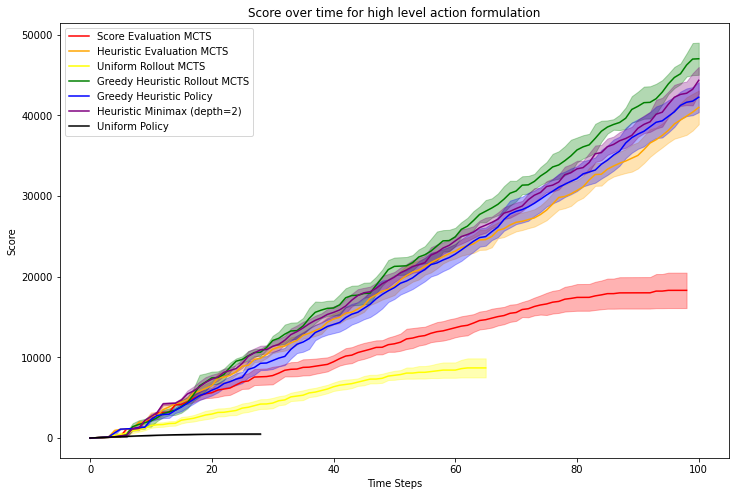
\includegraphics[width=\columnwidth]{HL.png}
  \caption{The results of running each configuration and baseline for 10 episodes (except for Monte Carlo tree search with greedy heuristic rollout, which was run for 5 episodes) with the high-level action formulation. Confidence bands are shown. The x-axis shows the time step, which is the same as the number of pieces placed in this case.}\label{fighl}
\end{figure}

As shown in Figure~\ref{fighl}, the uniform policy baseline agent performed terribly, not even surviving for 100 timesteps. The uniform rollout Monte Carlo tree search performs better in both score and survival, but not as well as the other configurations and baselines. It is hard to see from the graph, but the agent actually never survived up to 100 timesteps during the trials. The tree search baselines, the greedy heuristic rollout Monte Carlo tree search, and heuristic evaluation Monte Carlo tree search configurations performed comparably, but seem to separate after some time, with the greedy heuristic rollout Monte Carlo tree search performing the best, followed by the minimax agent, followed by the greedy heuristic policy, followed by the heuristic evaluation Monte Carlo tree search.

\begin{figure}[t]
  \centering
  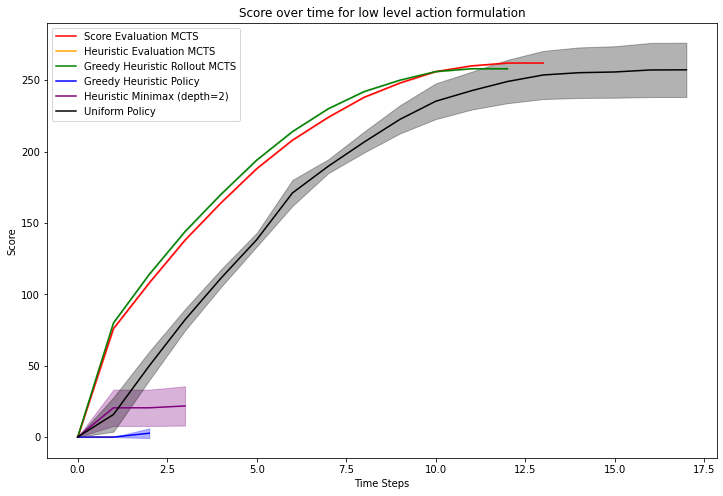
\includegraphics[width=\columnwidth]{LL.png}
  \caption{The results of running each configuration and baseline for 10 episodes (except for Monte Carlo tree search with greedy heuristic rollout, which was run for 5 episodes) with the low-level action formulation. Confidence bands are shown. The x-axis shows the number of pieces placed, not the number of low-level actions performed.}\label{figll}
\end{figure}

As shown in Figure~\ref{figll}, every agent performed terribly under the low-level action formulation, unable to place 100 pieces before losing or timing out. None of them cleared a line since the maximum score was under 1000, which is approximately the score for clearing a single line. The only score earned was from pieces falling and soft/hard drops. The two best-performing agents were only marginally better than the random baseline, and the simple tree search baselines were far worse than even the random baseline. Even the high performers lose before placing 100 pieces. I was not able to record results for the uniform rollout Monte Carlo tree search configuration because it kept getting caught in an infinite loop. I was not able to find the bug that caused this.

Heuristic Evaluation monte carlo tree search isn't visible on the graph. It never put down a piece. It stalled for all 1000 actions. That configuration as well as the simple tree search baselines all timed out after 1000 actions. They didn't terminate naturally.

\section{Conclusion}

\subsection{Summary and Discussion of High Level Action Formulation}

It seems strange that the heuristic evaluation monte carlo tree search agent performs worse, but it actually makes sense considering the nature of the heuristic. This heuristic essentially measures how ``messy'' the grid is. It penalizes for stack height, bumpiness, and holes. These are all things that usually increase when a piece is placed. In other words, as more pieces are placed, the grid gets ``messier''. Let's consider what would happen in Monte Carlo tree search with heuristic evaluation if we performed 45 iterations, one more than the number of actions:

Each action would be tried once after 44 iterations. The next iteration would select the action which led to the state with the highest heuristic score. Then, some action will be taken from that node in expansion, and it will be evaluated. Since this new node contains a state that is the result of adding a piece to the previous one, its heuristic score will likely be lower than its parent's. Then, this score will be backed up through the state-aciton node that used to be the most promising. This will bring its average down, possibly enough that it would be below what was the second-best action before the 45\textsuperscript{th} iteration. This means the agent would perform worse than the greedy heuristic policy in most situations.

This reasoning extends to a larger number of iterations. Nodes which look promising are explored, which causes their value to be averaged against lower values of future states, which make them look worse. I believe this is the cause for the lower performance. The minimax baseline doesn't have this problem because it only compares states that are the same number of pieces in the future. The Monte Carlo tree search agent has this problem because the search tree ends up unbalanced. It would be interesting to see the shape of the search tree and how many simulations have been run for the chosen action.

It is also unsurprising that the score evaluation Monte Carlo tree search configuration doesn't perform well. It takes at least three pieces to clear a line, usually more. This means comparing different long-term plans that span many line clears requires a significant search depth. With 150 iterations, the maximum selection depth with no exploration is about \(\frac{150}{44} \approx 3\), which isn't enough to meaningfully plan or compare plans. The agent seems to be capable of performing some line clears, but it doesn't seem like it can plan beyond that. Furthermore, excluding line clears, the scores for two different actions are usually very similar. In the high-level action formulation, the agent always hard drops after positioning a piece, which rewards some score. Thus, unless the agent plans very far ahead, it will not intentionally keep a ``clean'' grid and will not survive long, as we see with this configuration not surviving to 100 timesteps in any of the trials.

\subsection{Summary and Discussion of Low Level Action Formulation}

The low-level action formulation demonstrated terrible performance compared to the high-level action formulation. I think the reason the simple tree search baselines performed worse than random is because they maximize a heuristic, which generally decreases after placing a piece. This causes the agent to stall, rather than placing a piece. Since pieces do not immediately lock when they touch the grid, it is possible to stall by moving the piece around forever. I believe the reason the simple tree search baselines place a few pieces is because they can't plan ahead and somehow get into a situation where they can no longer stall, whereas the heuristic evaluation Monte Carlo tree search may be planning far ahead enough to avoid this. I do not know how it is possible to get into a situation where you cannot stall, since the player should always be able to rotate or move in some direction.

The uniform random baseline survived longer than the score evaluation and greedy heuristic rollout Monte Carlo tree search configurations, but scored less. I think this is because those Monte Carlo tree search agents immediately hard drop, whereas the uniform policy may move around for some before hard dropping. This means the stack doesn't grow quite as quickly, since some pieces aren't stacked right on top of each other.

I expected much better performance out of the score evaluation Monte Carlo tree search under the low-level action formulation. Since the algorithm runs for 150 iterations under an action formulation with just seven actions, I expected deep and higher-quality planning. However, the agent always immediately hard-drops. It doesn't see that it would survive longer by moving the piece over before hard-dropping to avoid stacking each piece on top of the last. Since immediately hard-dropping is what we'd expect from an agent greedily optimizing score, it looks like the agent isn't planning well enough to realize that the greedy policy isn't optimal. I should have tried different values of \(c\) for UCT to see if a better balance of exploration and exploitation would improve performance, but I didn't have time to run these experiments.

\subsection{Problems with Methods}

It is misleading to keep the simple tree search depth and number of Monte Carlo tree search iterations the same between both action formulations. Minimax sees \(b^{d}\) different states in a search, where \(b\) is the number of actions and \(d\) is the search depth. Monte Carlo tree search, however, sees exactly \(n\) states (during selection), where \(n\) is the number of iterations performed. \(d\) is kept the same, but the number of actions went from 44 to seven, so minimax sees far fewer states. Regardless, since the heuristic minimax agents stall under the low level formulation anyway, this doesn't matter.

Monte Carlo tree search configurations that use evaluation instead of rollout have some subtle biases for this problem. Score monotonically increases over time. For the score evaluation configuration, this effectively leads to an added bias towards exploitation during selection because nodes which have been more deeply selected have experienced states further into the future, which have higher scores than states in the past. When a state gets recursively selected, its estimated value will either stay the same or increase. This makes it more likely to be selected in the next iteration. The opposite happens for the heuristic, which usually decreases over time. This leads to an added bias for exploration.

\subsection{What I Learned}

During this project, I learned what it's like to do a full research project in AI. I learned about running experiments and actually measuring things to see if my intuitions and vague senses of performance were correct. This project started as a hobby project a few years ago where I implemented human and AI-playable \tetris{} and a simple heuristic minimax agent to play it. I just watched it run to judge it and was satisfied with that. Now, with this project, I actually ran experiments and measured performance.

Another thing I learned was what it's like to revisit an old project and pick it up again. I usually abandon old hobby projects and never work on them again once I achieved what I wanted to with them. I wrote this a few years ago, and I have changed a lot since then, so it was interesting to see my old habits. It was also interesting to see what the pain points were for figuring out what was going on in my code and fixing bugs that I found after revisiting. I learned what kind of documentation is important and how to write code that is easier to understand.

I also learned what it's like to write a paper in a research format, in \LaTeX{} with a template, which was interesting.

\end{document}
